\documentclass{report}
\usepackage[margin=1.25in]{geometry}
\usepackage{hyperref}
\usepackage{amsmath}
\usepackage{amssymb}
\usepackage{amsthm}
\usepackage{listings}
\usepackage{parskip}
\usepackage{graphicx}
\usepackage[center]{caption}

\newcommand\imageheight{10cm}

\newtheorem{thm}{Theorem}
\title{+/ Drawings}
\author{Varik Valefor}
\begin{document}
\maketitle{}
\tableofcontents{}
\chapter{Abstract}
This document contains some recent drawings which are created by VARIK VALEFOR, as well as some information regarding such drawings.

The word ``some'' is used because there exists a recent drawing which is created by VARIK VALEFOR $l$ such that $l$ is intentionally omitted from this document.  Examples of such drawings include VARIK's pornographic drawings.
\chapter{20200414042645-03}
\begin{figure}[ht]
	\centering
	
\includegraphics[height=\imageheight]{20200414042645-03/20200414042645-03.jpg}
	\caption[center]{The test drawing which has no ``true'' title.}
\end{figure}
\section{The Original Description of the Drawing}
This drawing was drawn to determine whether or not the use of computer mice as drawing tools is viable, and to determine whether or not GIMP is actually a terrible program; when drawing this image, that GIMP is a horrible computer program became very apparent, as did the computer mouse's viability as a drawing tool.

Dickcissels are cool.
\section{Watermarking}
VARIK finds that the watermarking of this drawing is a bit excessive\ldots especially when considering VARIK's having released relatively low-resolution unwatermarked versions of ``20200414042645-03''.
\begin{figure}[ht]
	\centering
	
\includegraphics[height=10cm]{20200414042645-03/20200414042645-03-uw.png}
	\caption[center]{A version of the drawing which lacks watermarking is revealed\ldots as is the absence of some fur texturing.  Gross.}
\end{figure}
\chapter{Proactive Security}
\begin{figure}[ht]
	\centering
	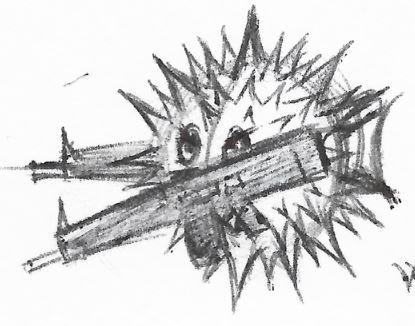
\includegraphics[height=10cm]{proactivesecurity/proactivesecurity.png}
	\caption[center]{We run OpenBSD here.  Don't even try it, punk.}
\end{figure}
\section{The Original Description of thhe Drawing}
The attached drawing is posted in response to the apparent lack of drawings which feature Puffy.

Puffy lacks eyebrows because someone forgot to add eyebrows.

The AA-12 is a cool gun.
\chapter{WESTERNUNIONSOFTHECOUNTRYWESTERNS}
\begin{figure}[ht]
	\centering
	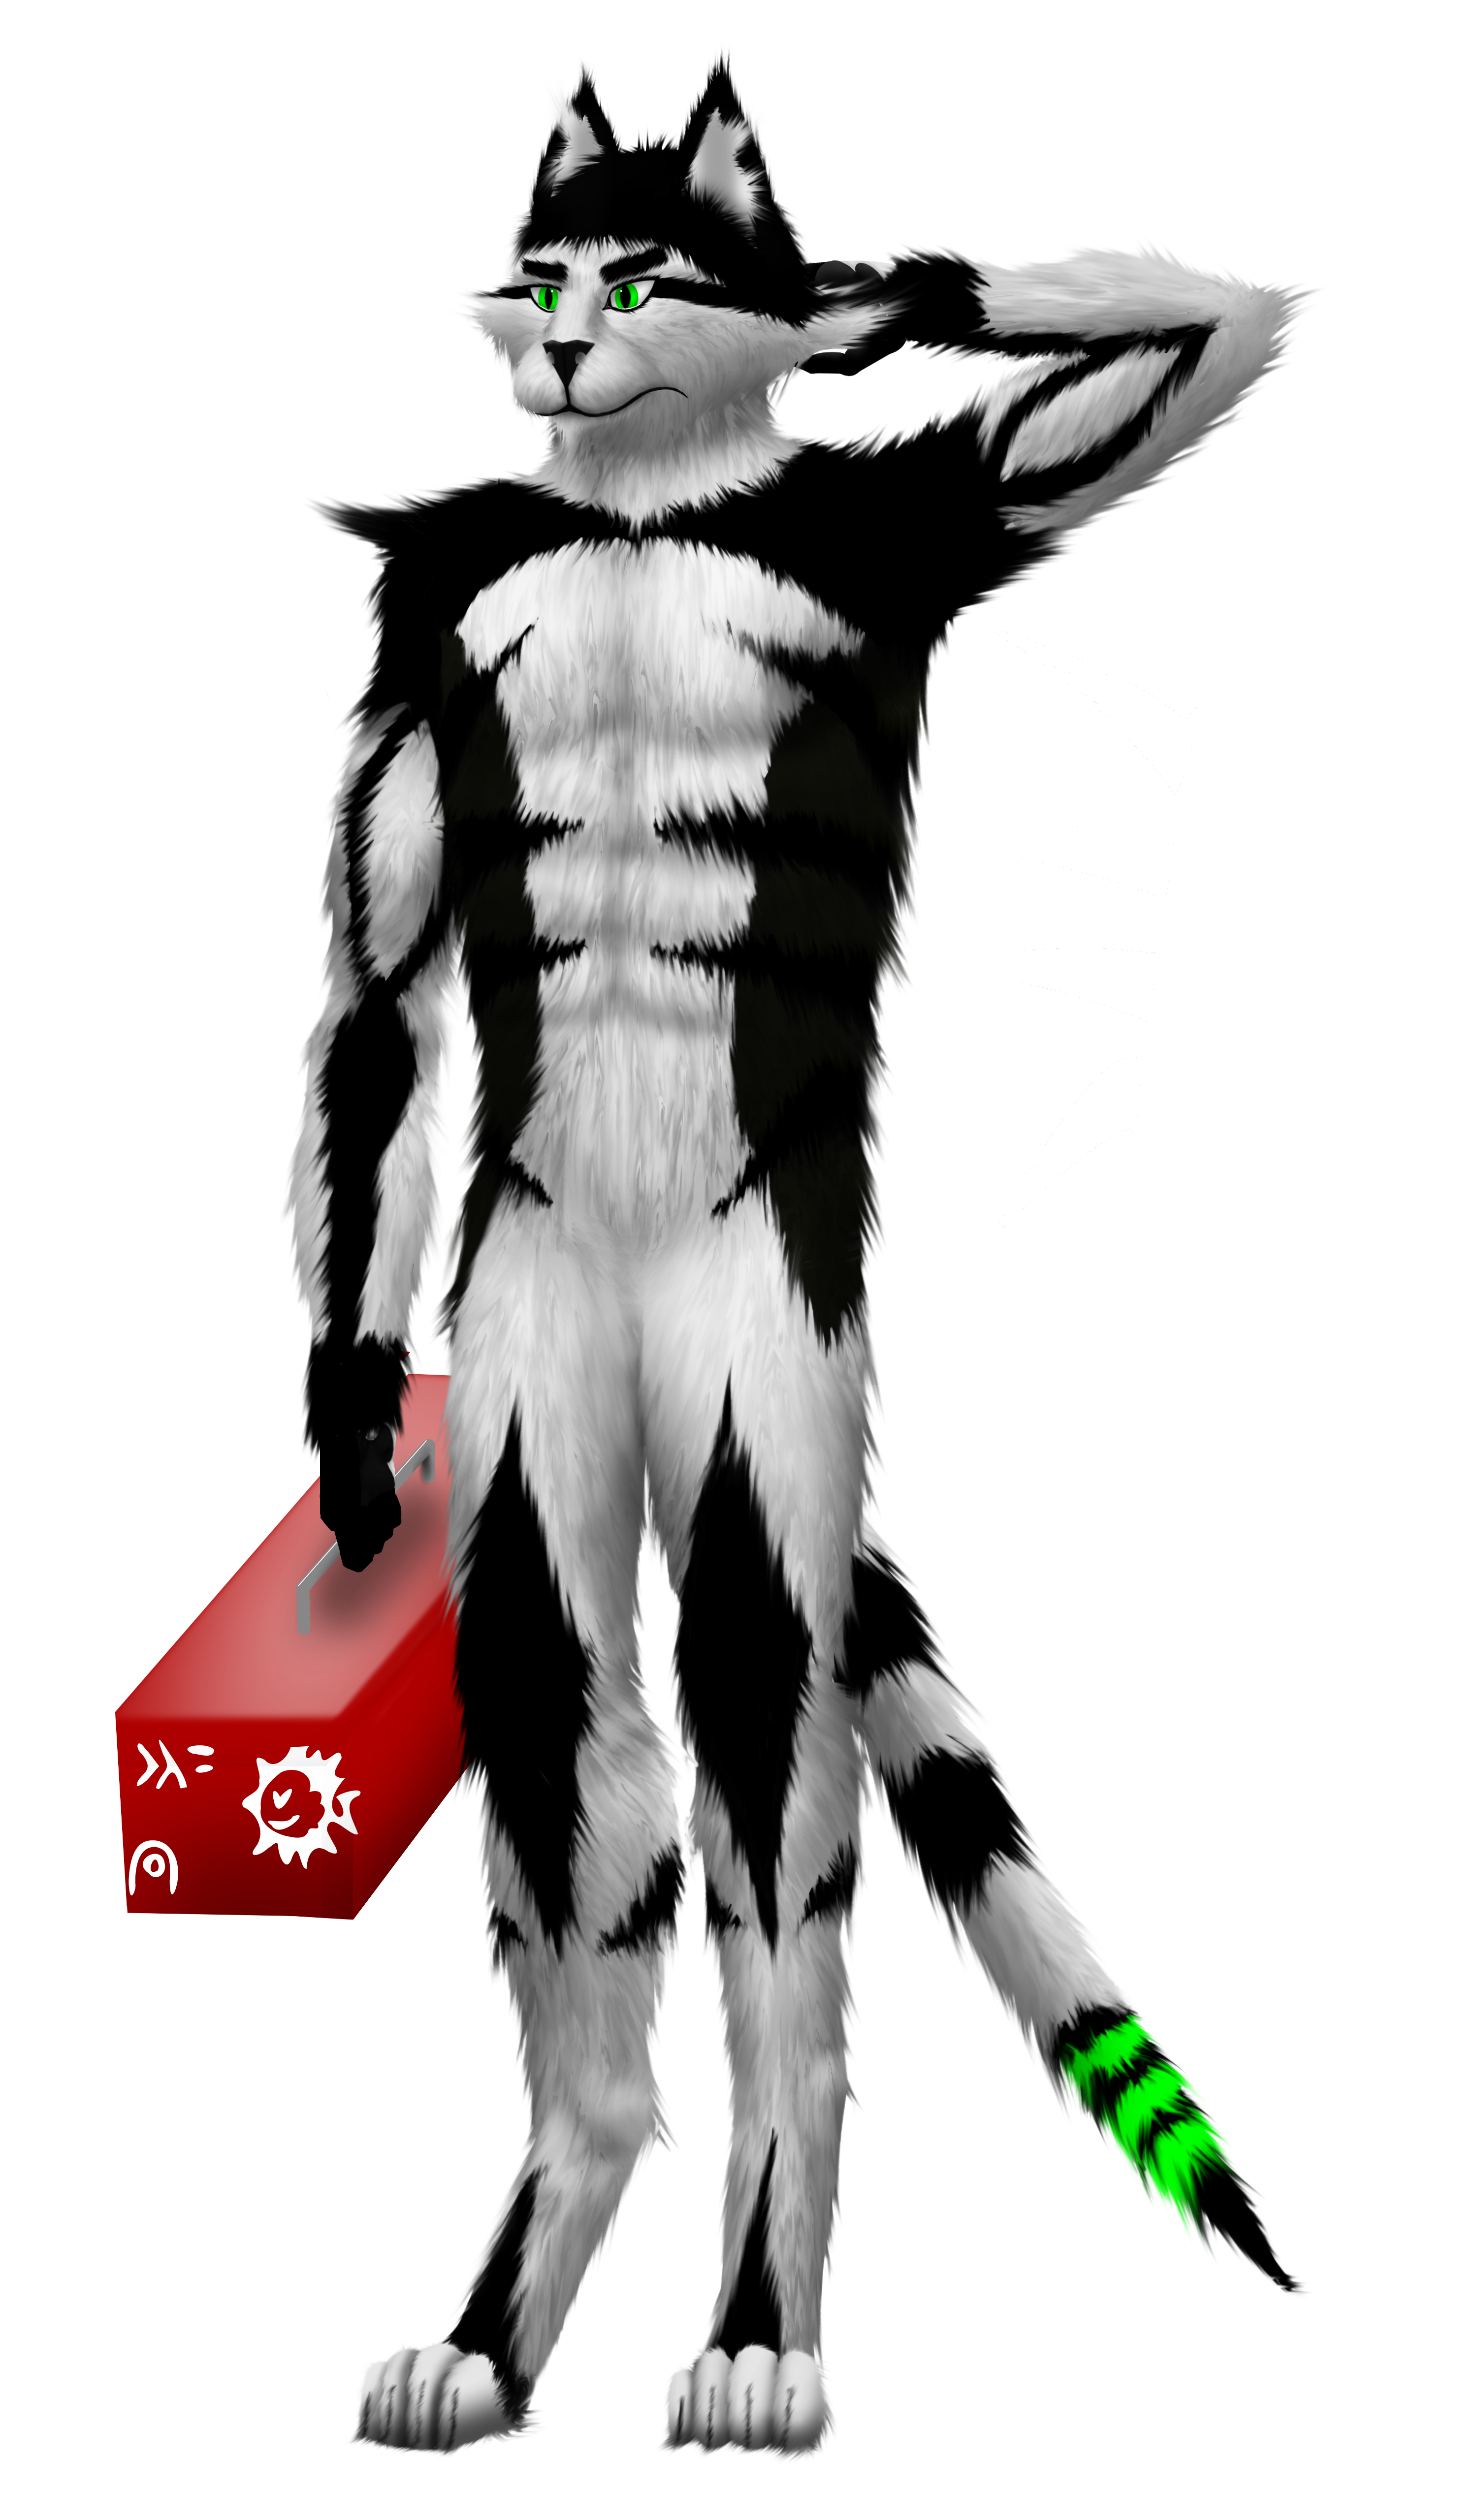
\includegraphics[height=\imageheight]{50x/toolbox/westernunionsofthecountrywesterns.png}
\caption{The actual drawing, as opposed to a bunch of text.}
\end{figure}
\section{The Original Description of the Drawing}
\subsection{A Successful ``Three-Quarters'' Thing}
After trying and struggling to draw VARIK's character in a ``three quarters'' pose for a decent period of time and taking rather long breaks between drawings, VARIK actually manages to somewhat decently draw VARIK's character such that VARIK's character is depicted in a ``three quarters'' pose.
\subsection{Watermarking and Licensing}
Additionally, this drawing is not \textit{too} obnoxiously watermarked.  However, this drawing is NOT released into the public domain.  VARIK retains the rights to this drawing, although this fact may change as time passes; as time passes, VARIK becomes increasingly friendly to the idea of releasing VARIK's drawings into the public domain.
\subsection{Tools Used}
This drawing is drawn using Krita, which VARIK quite dislikes.

During the creation of this drawing, Krita is all but unusably slow, as Krita manages to make layers invisible in the short timespan of approximately thirty seconds.  Partially as a result of this slowness, VARIK may create future drawings using CLIP STUDIO PAINT EX; VARIK owns a copy of CLIP STUDIO PAINT EX and finds that CLIP STUDIO PAINT EX is superior to Krita by nearly every metric.  VARIK's appreciation for WINE on FreeBSD manages to grow even greater.

GIMP is also used for a short while; however, after being in development for multiple decades, GIMP lacks some basic features which VARIK uses, e.g., clipping masks.  As such, VARIK completes this drawing with Krita.
\subsubsection{Yes, Open-Source Stuff \textit{can} be All Right}
The ``open-source'' idea is cool\ldots but can generate some real shit.  ``Critics can fix the software'' is a crap excuse, as not all users are computer programmers.  Additionally, nearly unmaintainable source code exists, and VARIK does not find that Krita's source code is particularly good.

These problems are mentioned because VARIK wishes to like Krita and GIMP\ldots but cannot actually like Krita and GIMP unless Krita and GIMP stop being frass.
\subsection{``Logos'' and Whatnot}
Determining the meanings of the ``logos'' which are present on the toolbox is left as a trivial exercise for the reader.  ``[L]ogos'' is written in inverted commas because some such things may not really be logos.
\subsection{On the Use of Version Control}
The history of this file may eventually be uploaded to GitHub; this file is tracked via Git, generating a fairly large repository.  However, this history \textit{may} be encrypted, as VARIK wishes to be able to reasonably easily provide evidence of VARIK's having created this drawing.
\subsection{Criticism}
As ever, decent criticism is strongly appreciated.  However, VARIK requests that such criticism is detailed; VARIK finds that the extent to which ``the shape of the fur does not match the shading of the arm'' is helpful is greater than the extent to which ``the fur looks bad'' is helpful, although both things can be helpful.
\subsection{Tools Used}
This description is written with the good ol' ed(1).
\section{Janky Abdominal Muscles}
In ``WESTERNUNIONSOFTHECOUNTRYWESTERNS'', VUNC's abdominal muscless are a bit misshapen.

This problem likely results from VARIK's cheesy method of adding VUNC's abdominal muscles.  This method involves adding muscles individually.
\section{Speedpaint}
A narrated video which depicts the creation of ``WESTERNUNIONSOFTHECOUNTRYWESTERNS'' is available at \url{https://diode.zone/w/vR9yipHTfuaH3SKPiEXFLm} and \url{https://vimeo.com/635651456}.  However, motherfucking heretics can also view the video at \url{https://www.youtube.com/watch?v=0wyF7okop64}.
\subsection{Crappy Video Quality}
The quality of the video portion of the narrated speedpaint is a bit cheesy.

This cheesiness likely results from VARIK's having used \textsc{ffmpeg}'s optionless AVI output to record the narrated video; when used without options, \textsc{ffmpeg}'s AVI output uses very lossy H.264 encoding.
\section{Lack of Fur Detail}
In this drawing, VUNC's fur lacks some fine detail.

Whilst drawing ``WESTERNUNIONSOFTHECOUNTRYWESTERNS'', VARIK fails to add the fine fur layer to the drawing.  This failure results in a drawing which contains only coarse fur texturing.
\chapter{HOLLYWOODFREAKSONTHEHOLLYWOODSCENE}
\begin{figure}[ht]
	\centering
	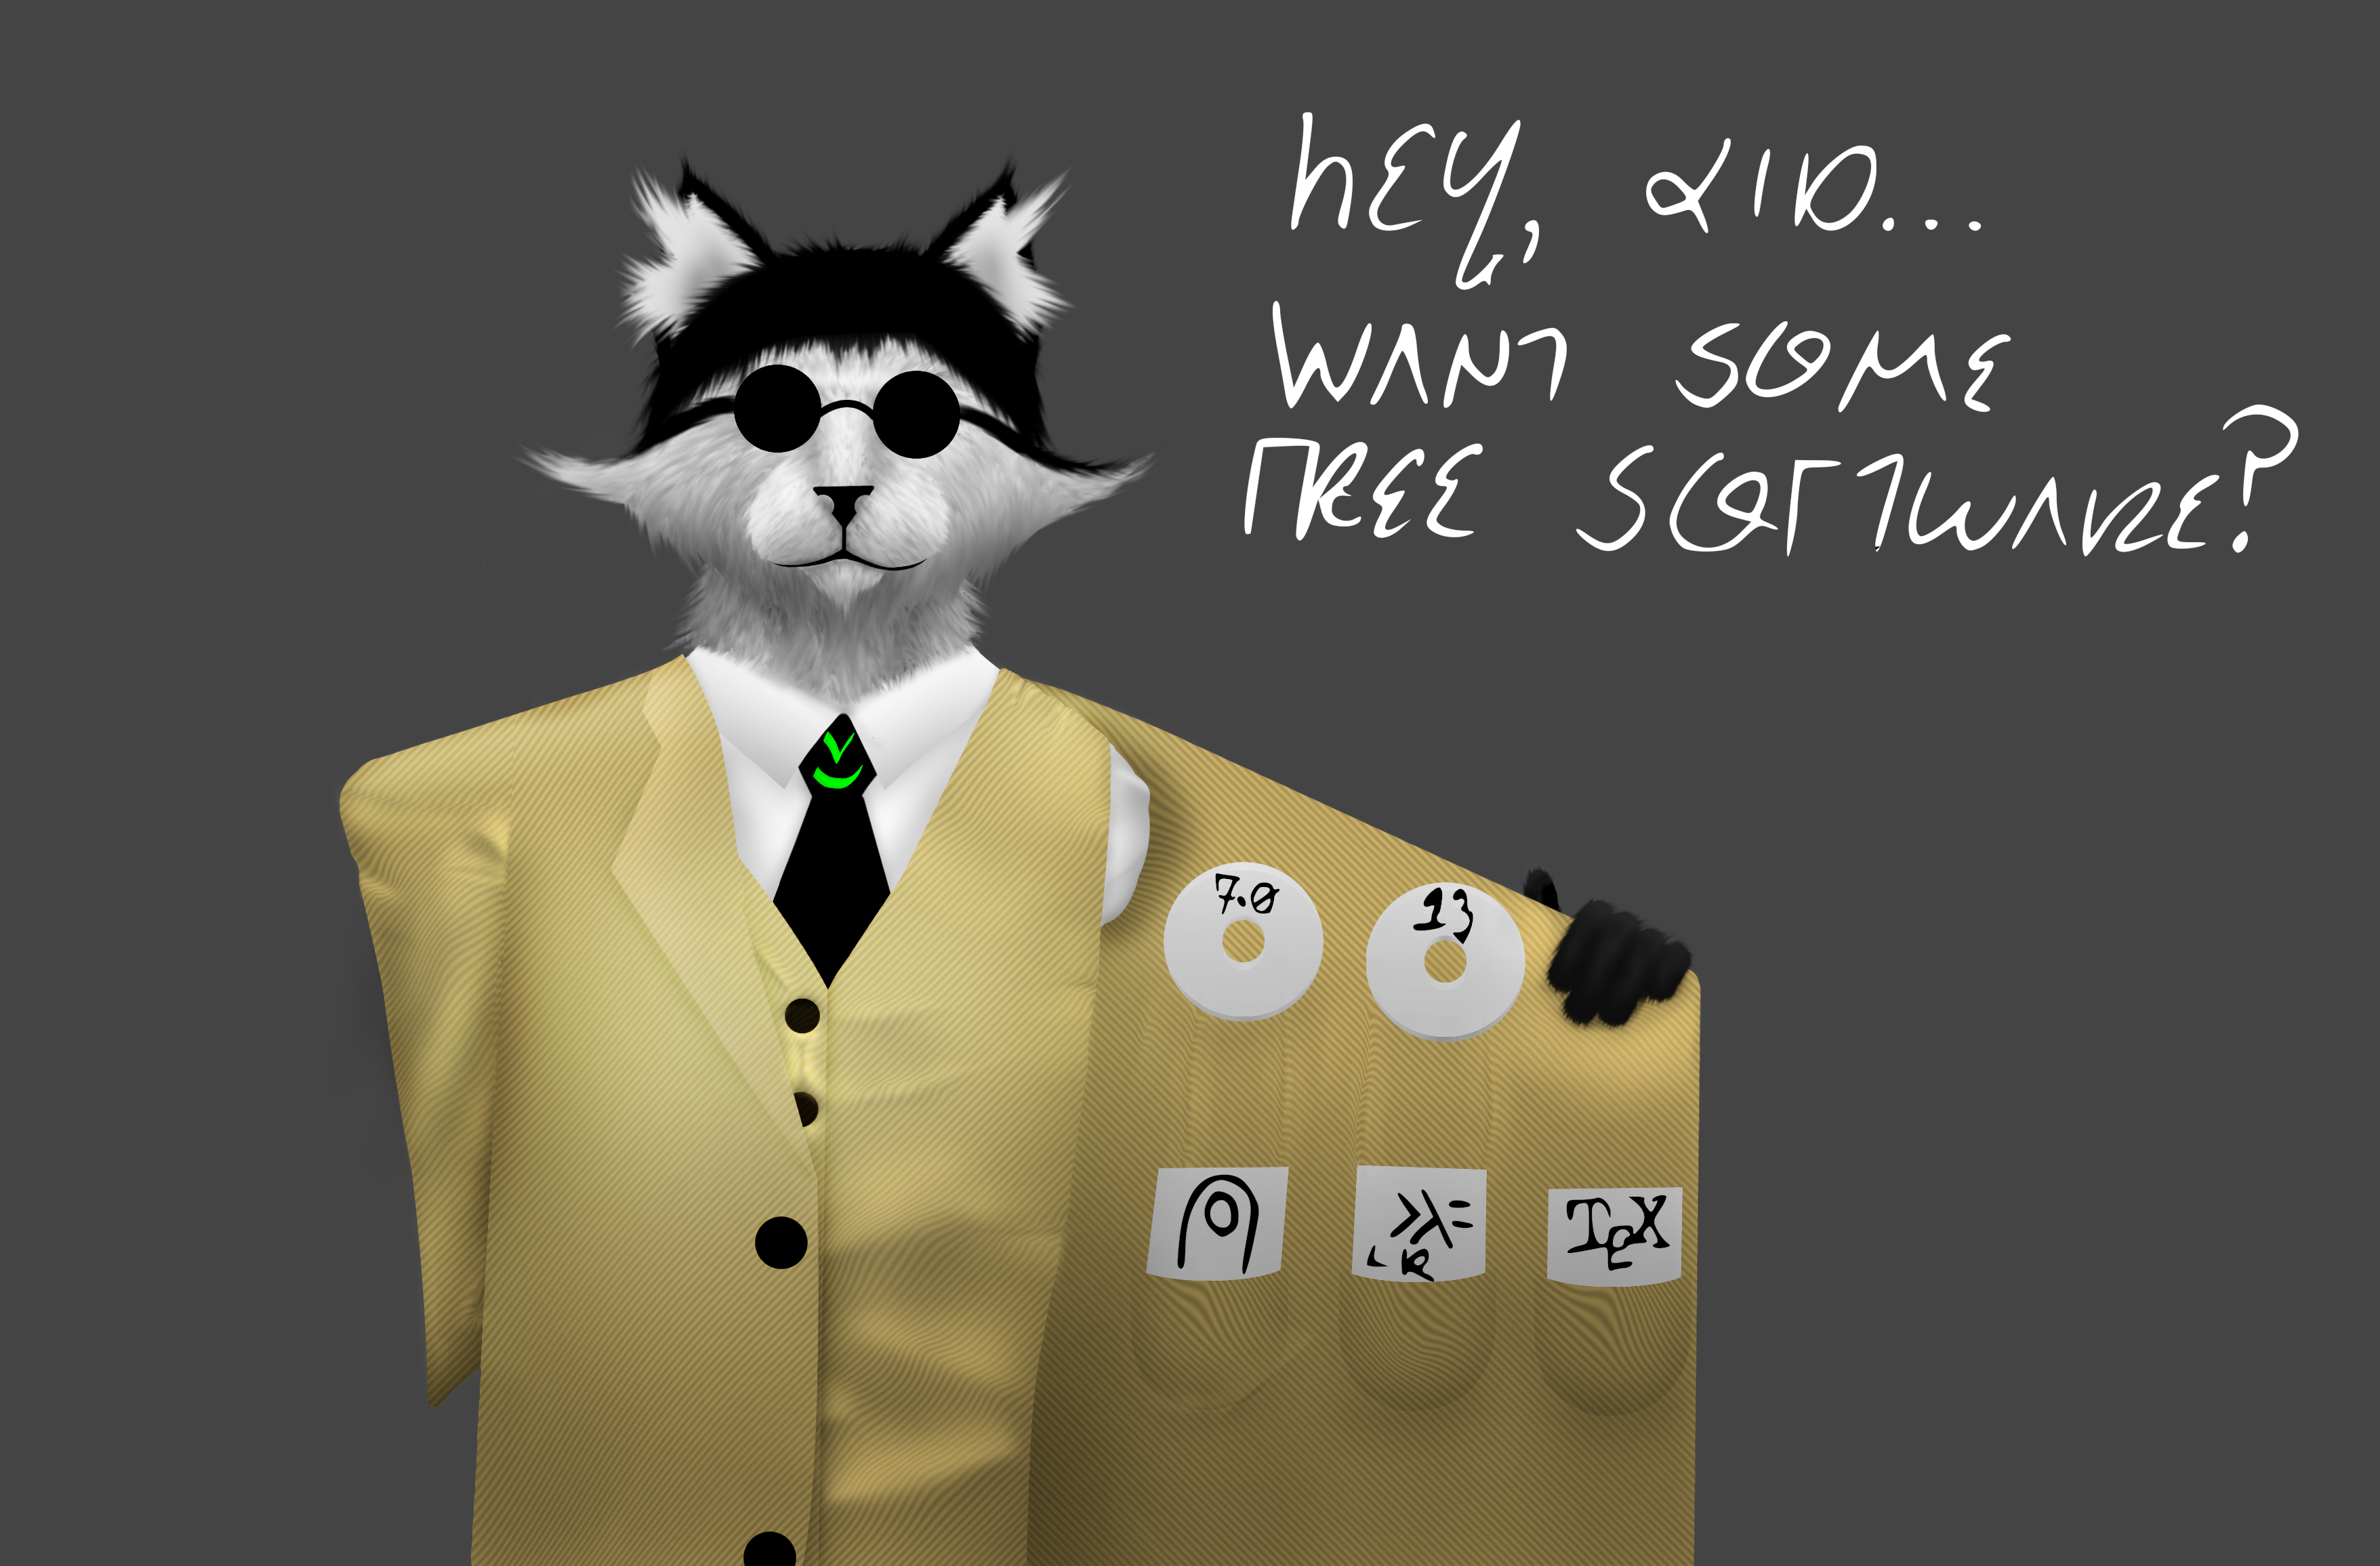
\includegraphics[height=\imageheight]{hollywoodfreaksonthehollywoodscene/hollywoodfreaksonthehollywoodscene.png}
	\caption[center]{``HOLLYWOODFREAKSONTHEHOLLYWOODSCENE''.}
\end{figure}
\section{The Original Description of the Drawing}
\subsection{A Cheesy-Ass Short Story}
Let there exist a man $J$.

$K$ denotes the depicted man.

In the middle of an arbitrary night, as $J$ walks down an arbitrary street and nears a power substation, $K$ appears from behind a bush and slowly approaches $J$.

Whilst $J$ appears rather surprised and unnerved, $K$ opens $K$'s coat and speaks the following words: ``Hey, kid\ldots want some free software?''

Determining whether or not $J$ ``takes up'' $K$'s offer is left as an exercise for the reader.
\subsection{Blah}
Another dumb joke is revealed!  In this case, the joke takes the form of a drawing which is called ``HOLLYWOODFREAKSONTHEHOLLYWOODSCENE''.

In addition to being a dumb joke, this drawing is VARIK's first \textit{real} attempt to draw fabric.
\subsection{The Contents of the Coat}
\subsubsection{Discs}
The ``7.0'' disc is an OpenBSD installation disc, and the ``13'' disc is a FreeBSD installation disc.  As of the publishing of this drawing, 7.0 and 13.0 are the most recent versions of OpenBSD and FreeBSD, respectively.
\subsubsection{Coat Pockets}
The reader can assume that the contents of the pockets of the coat are specifications and compilers of the programming languages whose ``logos'' are mentioned.  ``[L]ogos'' is written in inverted commas because one such ``logo'' is not an established logo but is a recognisable feature of the programming language which this ``logo'' represents.
\subsubsection{On the Amount of Stuff}
Whilst conceptualising this drawing, VARIK intends to mention a relatively great number of softwares.  However, there exists an idea such that this idea does not immediately come to fruition.  A ``deluxe'' version of this drawing may eventually be created.
\subsection{Criticism}
As ever, criticism regarding this drawing is appreciated.
\subsection{Tools Used}
This drawing is drawn using GIMP\@.

This description is written using ed(1).
\section{Two-Dimensional Appearance of Clothing}
Several men claim that in ``HOLLYWOODFREAKSONTHEHOLLYWOODSCENE'', VUNC's clothing lacks depth and appears to be paper or something.

VARIK agrees with this assessment.

Luckily, the idea of wearing a paper suit which lacks a back is damn funny.
\section{Shading of Discs}
VARIK finds that the discs resemble paper cut-outs, as opposed to optical discs.  This problem may result from the discs' complete opacity.
\chapter{BROKEDOWNOUTINADITCHOFOLDRUBBISH}
\begin{figure}[ht]
	\centering
	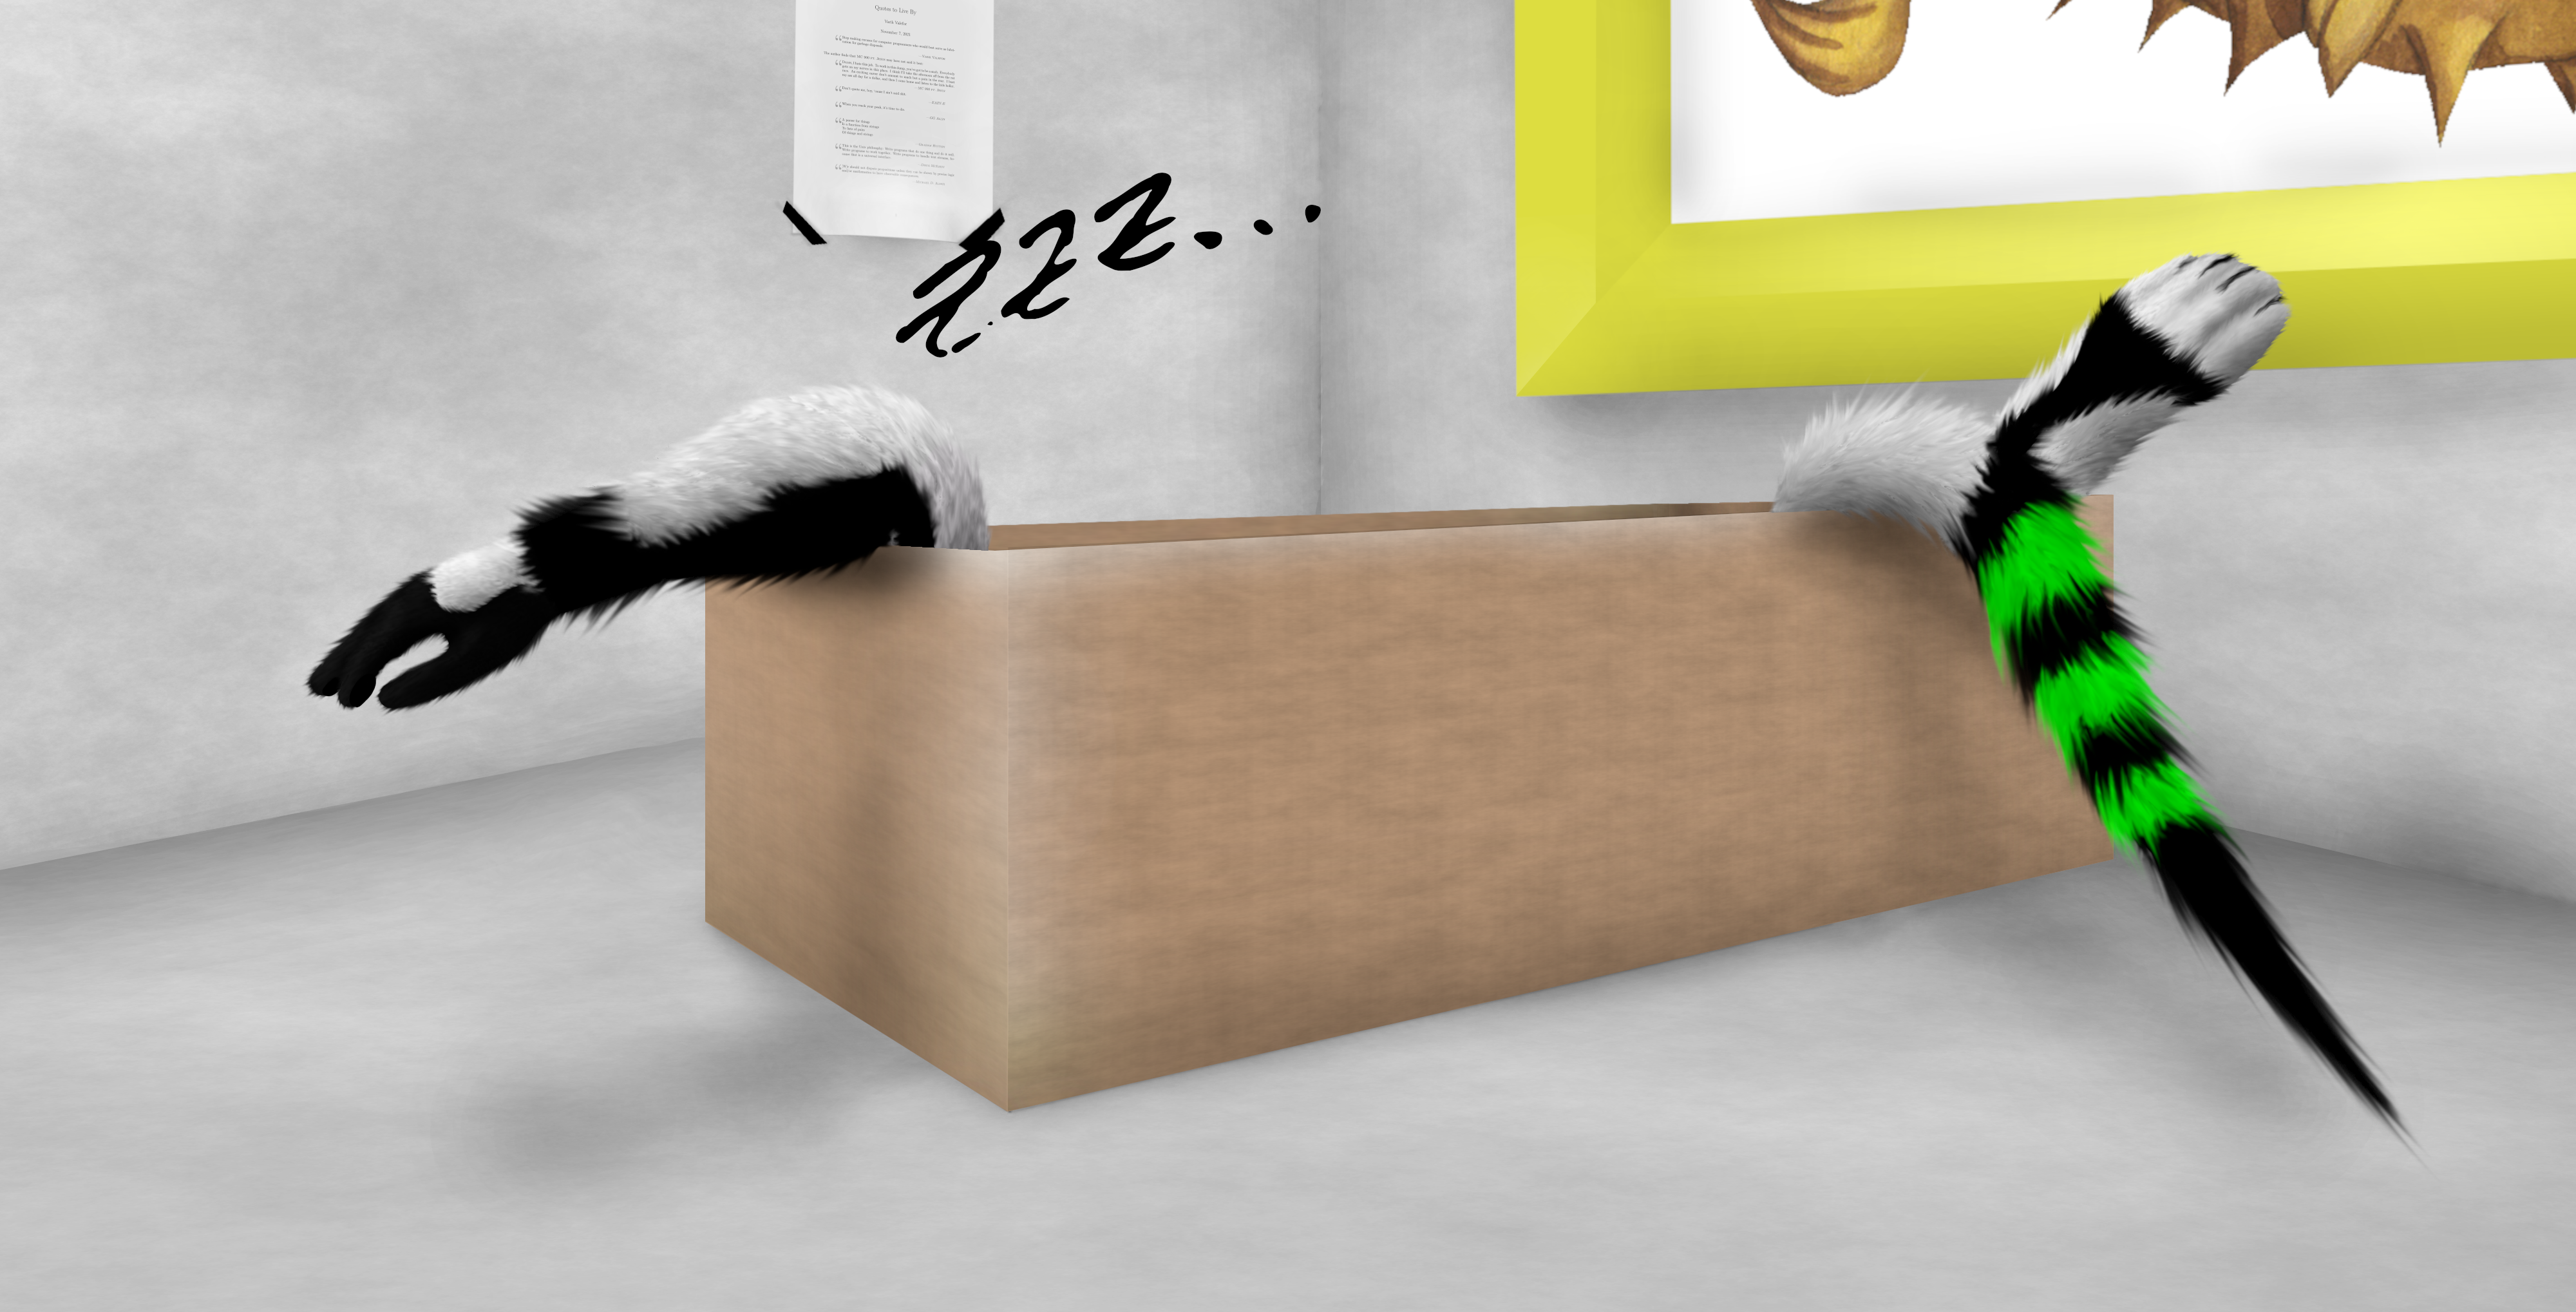
\includegraphics[width=\textwidth]{brokedownoutinaditchofoldrubbish/brokedownoutinaditchofoldrubbish.png}
	\caption[center]{This figure is the drawing.  Is a photograph of a ham sandwich or something expected?  Have some sense, foo'.}
\end{figure}
\section{The Original Description of the Drawing}
A new drawing is revealed!

\subsection{``Proper'' Background\ldots and Jokes}
This drawing, which is called ``BROKEDOWNOUTINADITCHOFOLDRUBBISH'', is VARIK's first published drawing which features a ``proper'' background, as opposed to a solid colour or some abstract thing.  Additionally, ``BROKEDOWNOUTINADITCHOFOLDRUBBISH'' includes a few jokes.

\subsection{On the Box}
The reader can assume that the cardboard box in which the character lies is reinforced such that this box is not deformed under minor weight.  The reader can also assume that the flaps of this box are folded inward or removed.

\subsection{Origins as an Inside Joke}
This drawing actually begins as an inside joke, as the box is originally adorned with some text which functions as an inside joke.  However, VARIK eventually concludes that this inside joke is not terribly amusing and removes the part of the drawing which qualifies as an inside joke.

\subsection{On ``ZZZ\ldots''}
The presence of ``ZZZ\ldots'' indicates that the character is snoring, which indicates that the character is sleeping.  But why in the hell is ``ZZZ\ldots'' the accepted transcription of snoring?

\subsection{Criticism}
As ever, criticism is appreciated.

\subsection{Weapons of Choice}
This drawing is created using GIMP\@.  The actual drawing work is done with a trackpad.

This description is written using ed(1).

Both GIMP and ed(1) are run on OpenBSD\@.
\chapter{DANCINGONTHEROOFSHOOTINGHOLESINTHEMOON}
\begin{figure}[ht]
	\centering
	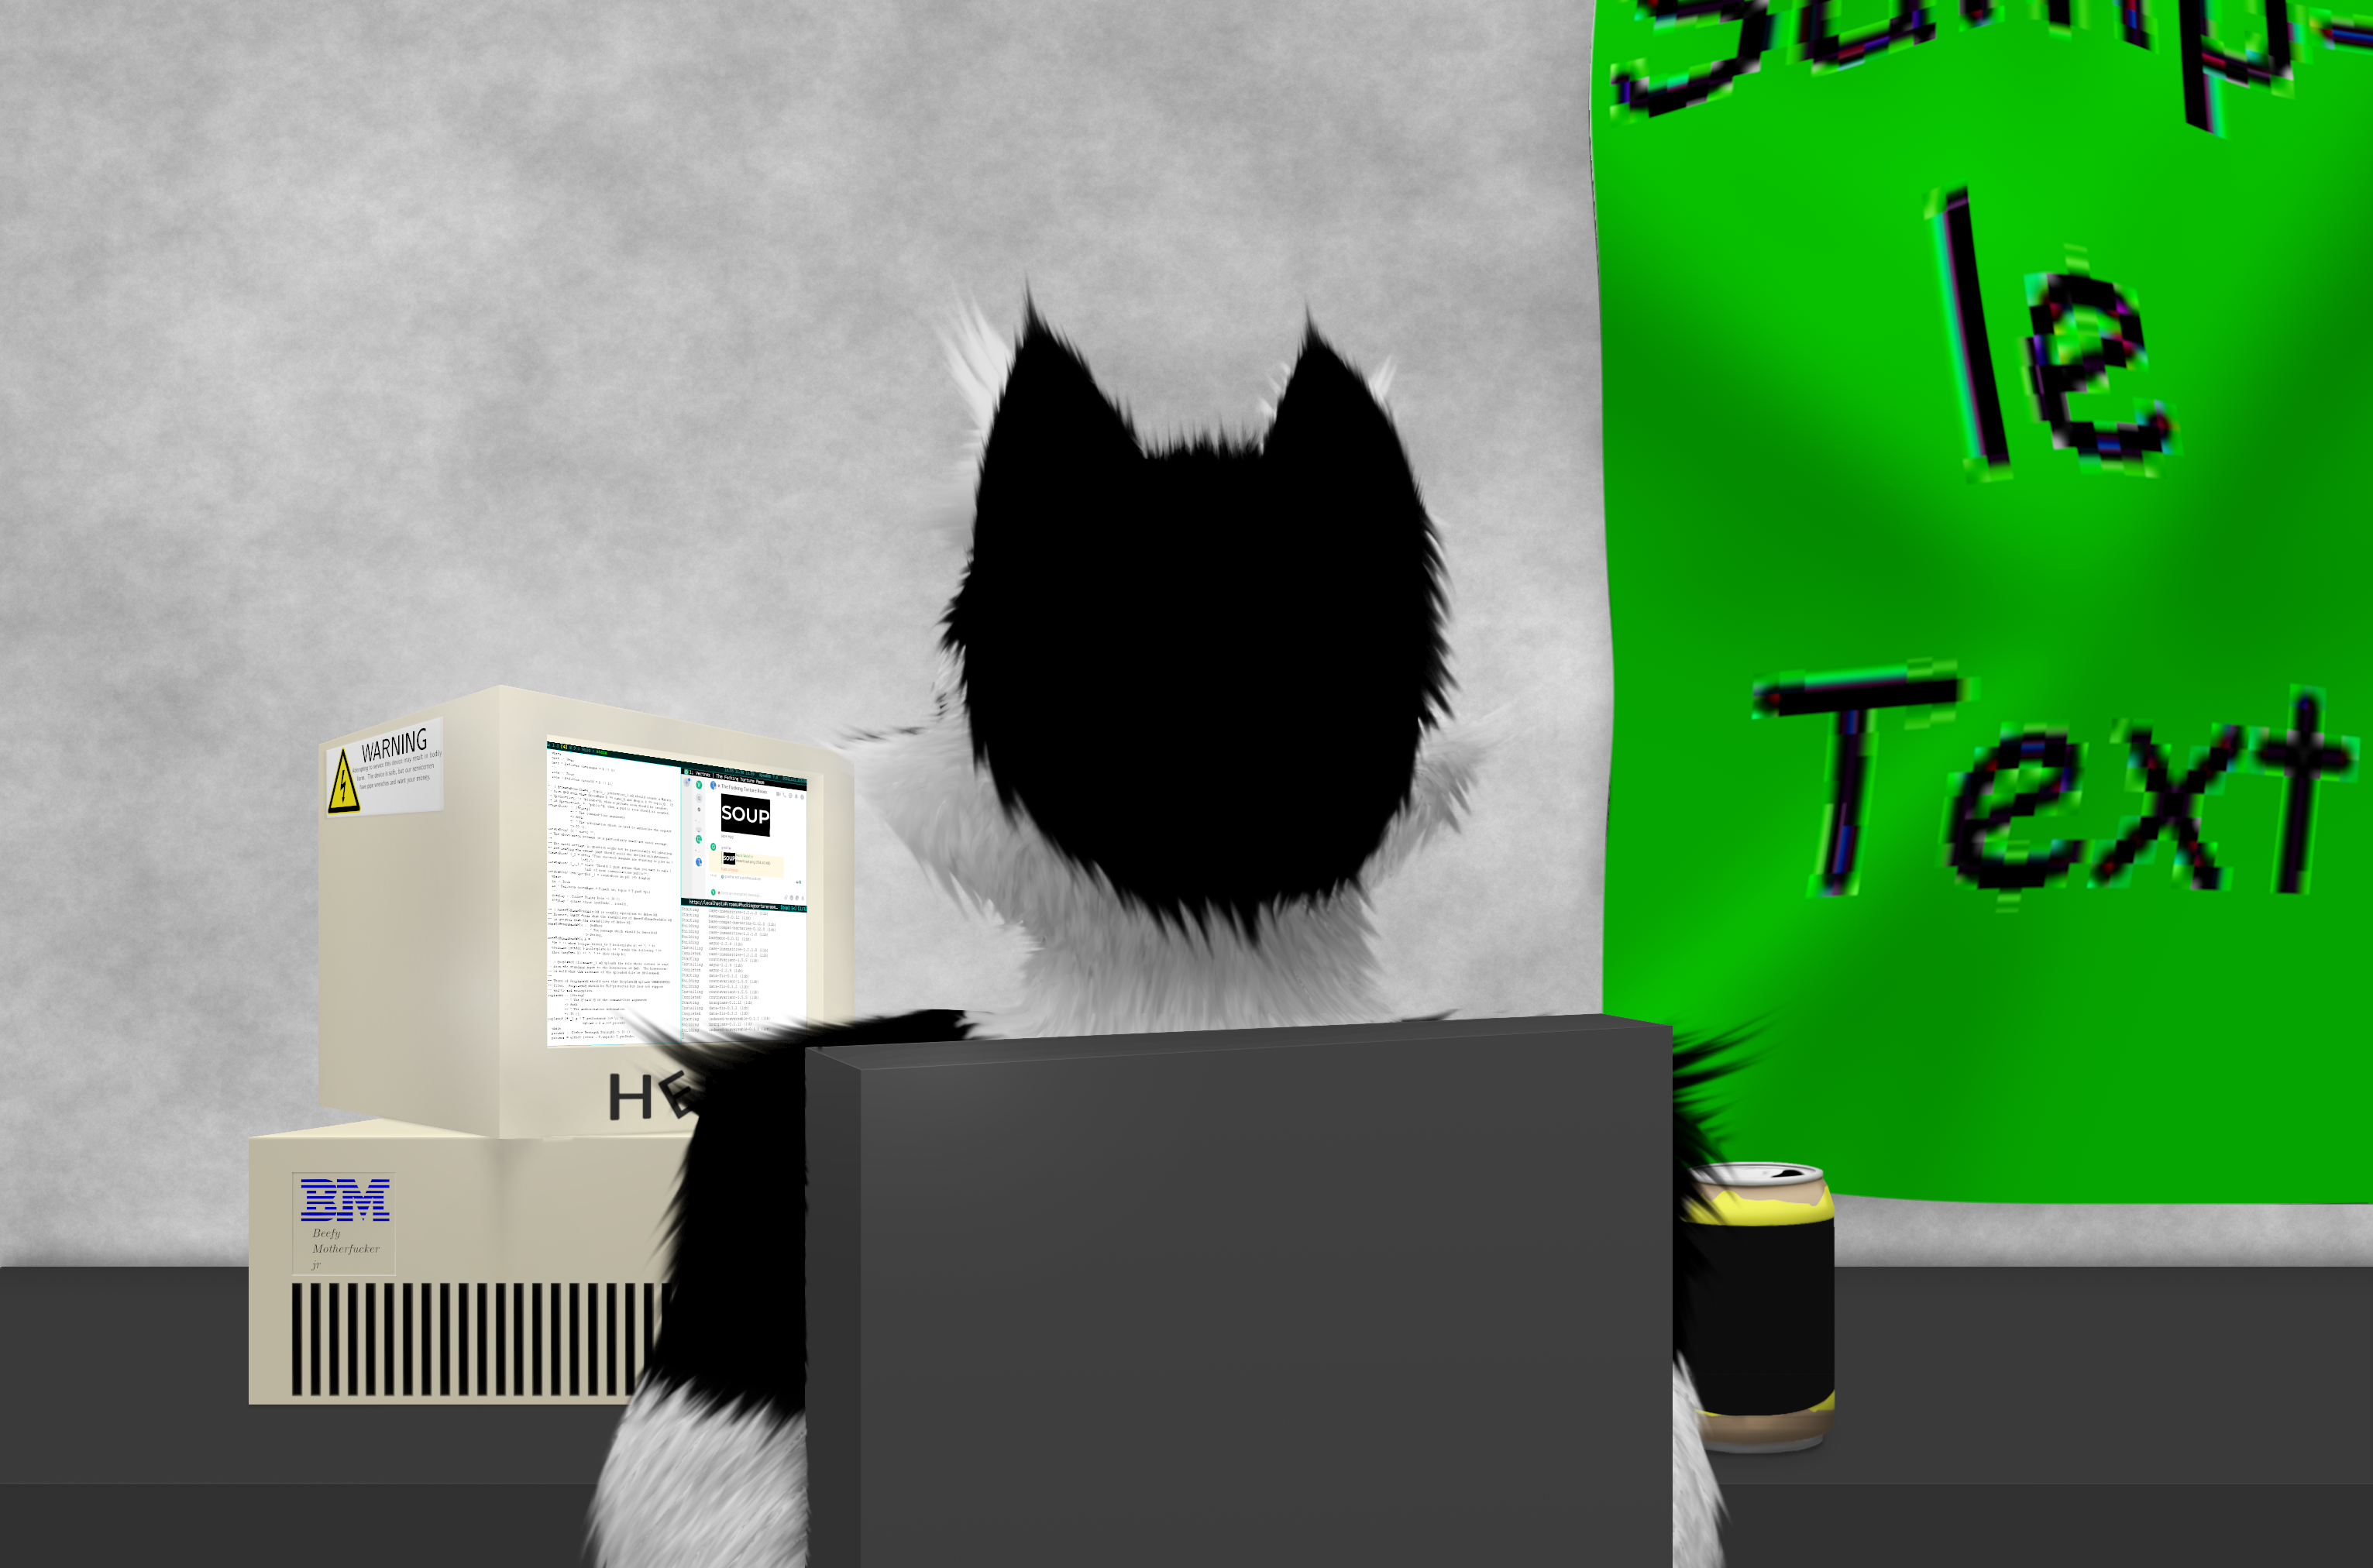
\includegraphics[width=\textwidth]{dancingontheroofshootingholesinthemoon/dancingontheroofshootingholesinthemoon.png}
\caption[center]{The full version of ``DANCINGONTHEROOFSHOOTINGHOLESONTHEMOON''.  To see every detail, use a magnifying glass\ldots or a microscope.}
\end{figure}
\section{The Original Description of the Drawing}
Yet another drawing is created!
In this case, the drawing depicts an everyday situation\ldots but is hopefully not too boring.

\subsection{Definitions}
Let ``VUNC'' denote VARIK's character.

\subsection{Executive Summary}
In this drawing, VUNC sits at a terminal and works on some tedious software-related stuff\ldots whilst reading terrible chatroom messages.
\subsection{Jokes and Whatnot}
Like VARIK's other drawings, this drawing features a decent number of jokes and references.  Explaining these jokes is left as an exercise for the reader.

However, in addition to some jokes, this drawing contains a small social commentary.  Describing this social commentary is \textit{also} left as an exercise for the reader.
\subsection{On ``SOUP''}
The stupid-looking ``SOUP'' image on the display is present because VARIK is uncertain of whether or not the original image can be included freely in the drawing.  To prevent a lawsuit or the threat of a lawsuit, a ``description'' of the possibly copyrighted image replaces the possibly copyrighted image.

``[D]escription'' is written in inverted commas because this ``description'' is not terribly descriptive.  A relatively descriptive description of the original image is ``a heavily-compressed photograph of a bowl of alphabet soup''.
\subsection{Warning Label}
The full text of the warning label is as follows:
\begin{quote}
	WARNING

	Attempting to service this device may result in bodily harm.  The device is safe, but our servicemen have pipe wrenches and want your money.
\end{quote}
\subsection{Keyboard}
In the depicted scene, VUNC uses a keyboard.  However, this keyboard is not visible, and VUNC's use of this keyboard could probably be relatively well indicated.
\subsection{Criticism}
As ever, criticism is welcomed.
\subsection{Licence}
This drawing is released in accordance with the CC BY-NC 4.0 licence.  The full text of this licence is available at \url{https://creativecommons.org/licenses/by-nc/4.0/legalcode}.
\subsection{Tools Used}
This drawing is created using GIMP\@.  GIMP is terrible but seems to be the best open-source drawing software.

This description is written using ed(1).

Both GIMP and ed(1) are run on OpenBSD\@.
\section{Chair}
The chair which VUNC uses lacks detail; the material of the chair is ambiguous.  The design of the chair is mostly style-based, as VARIK strongly likes brutalist architecture; however, regardless of the style, the chair just looks a bit cheesy.
\chapter{ITHINKWEREGOINGCRAZY}
\begin{figure}[ht]
	\centering
	\includegraphics[height=10cm]{ithinkweregoingcrazy/ithinkweregoingcrazy.png}
	\caption[center]{``ITHINKWEREGOINGCRAZY''.}
\end{figure}
\section{The Original Description of the Drawing}
BLOCKED BY SHODAN LEVEL SECURITY\@.
\subsection{``What the Hell am I Looking At?''}
This drawing depicts VARIK's character's being connected to some cables and having a neutral facial expression a la \textit{System Shock}'s SHODAN\@.
\subsection{Timing}
December apparently has at least one (1) drawing, as well.
\subsection{History}
\subsubsection{The Sketch}
Approximately fifteen (15) quintillion years ago, VARIK reveals a sketch which features VUNC hooked up to some cables a la \textit{System Shock}'s SHODAN\@.
\subsubsection{The First Attempted Conversion}
In early 2021, VARIK begins to convert this sketch into a ``proper'' drawing.  However, before VARIK backs up the drawing, VARIK accidentally deletes the master boot record of the hard disk drive of VARIK's terminal.  As a result of this mistake, the original version of the ``proper'' drawing is probably lost forever.
\subsubsection{The Second Attempted Conversion}
On 20210411, VARIK begins the process of converting the sketch into a ``proper'' drawing by adding the un-furred outlines of VUNC to a Scalable Vector Graphics file.  This process is finished with minimal ``hiccups''.
\subsubsection{Attempting to Add Detail}
Circa 20210602, VARIK converts the aforementioned SVG file into an XCF file and begins to add some detail.  For some reason, such detail is added before the cables are added.

Although few ``real'' problems are encountered, VARIK does not particularly care for the end result of the addition of such detail and pauses the creation of the drawing.
\subsubsection{Successfully Adding Detail}
On 20211127, VARIK resumes the creation of the drawing.  VARIK encounters few ``real'' problems but again concludes that GIMP can be a real turd\ldots figuratively.
\subsubsection{Finishing the Drawing}
On 20211201, VARIK declares that this drawing is finished.
\subsection{On this Drawing's Nature as an Amalgamation}
\textit{System Shock}'s SHODAN SHODAN serves as the direct inspiration of the creation of the SHODAN-``inspired'' parts of this drawing.  However, VARIK uses no particular SHODAN design as a reference whilst creating this drawing; VARIK bases this drawing upon a mental combination of SHODAN's \textit{System Shock} and \textit{System Shock 2} designs.
\subsection{Criticism}
As ever, criticism is welcomed.
\subsection{Licence}
This drawing is released in accordance with the CC BY-NC 4.0 licence.  The full text of this licence is available at \url{https://creativecommons.org/licenses/by-nc/4.0/legalcode}.
\subsection{Tools Used}
This drawing is created using GIMP\@.  GIMP is terrible but at least beats Krita.

This description is written using ed(1).

Both GIMP and ed(1) are run on OpenBSD\@.
\section{Eyestrain}
There exists a subset of all men $K$ such that for all $a \in K$, $a$ claims that $a$'s viewing of ``ITHINKWEREGOINGCRAZY'' results in the eyestrain of $a$.  VARIK suspects that men of $K$ are exaggerating things or have some weird eye problem; VARIK is incapable of finding any particular source of the eyestrain.
\section{Reception}
In short, ``ITHINKWEREGOINGCRAZY'' is relatively unpopular\ldots possibly because the ``source material'' of ``ITHINKWEREGOINGCRAZY'' is a bit obscure.
\subsection{Description of Reception}
The mean warmth of the reception of ``ITHINKWEREGOINGCRAZY'' is less than the mean of the warmths of the receptions of all drawings which VARIK creates.
\subsection{Possible Cause of Lukewarm Reception}
VARIK suspects that the relatively lukewarm reception of ``ITHINKWEREGOINGCRAZY'' may be a result of the relatively obscure nature of ``ITHINKWEREGOINGCRAZY''.
\begin{thm}
``ITHINKWEREGOINGCRAZY'' likely has a lukewarm reception.
\end{thm}
\begin{proof}
	${}$

	For all things $a$, for all drawings $b$, for all men $m$, $b$ is a parody of $a$ only if ($m$ fully understands $b$ only if $m$ is familiar with $a$).

	For all drawings $b$, few men fully understand $b$ only if $b$ likely has a lukewarm reception.\footnote{The reader should probably take this statement with the proverbial grain of salt.}

	Few men are familiar with \textit{System Shock}.\footnote{``Few'' may be an understatement.}

	``ITHINKWEREGOINGCRAZY'' is a parody of \textit{System Shock}.

	Therefore, ``ITHINKWEREGOINGCRAZY'' likely has a lukewarm reception.
\end{proof}
\end{document}
